% This must be in the first 5 lines to tell arXiv to use pdfLaTeX, which is strongly recommended.
\pdfoutput=1
% In particular, the hyperref package requires pdfLaTeX in order to break URLs across lines.

\documentclass[11pt]{article}
\DeclareUnicodeCharacter{FF0C}{,}


% Change "review" to "final" to generate the final (sometimes called camera-ready) version.
% Change to "preprint" to generate a non-anonymous version with page numbers.
\usepackage[final]{acl}

% Standard package includes
\usepackage{times}
\usepackage{latexsym}

% For proper rendering and hyphenation of words containing Latin characters (including in bib files)
\usepackage[T1]{fontenc}
% For Vietnamese characters
% \usepackage[T5]{fontenc}
% See https://www.latex-project.org/help/documentation/encguide.pdf for other character sets

% This assumes your files are encoded as UTF8
\usepackage[utf8]{inputenc}

% This is not strictly necessary, and may be commented out,
% but it will improve the layout of the manuscript,
% and will typically save some space.
\usepackage{microtype}

% This is also not strictly necessary, and may be commented out.
% However, it will improve the aesthetics of text in
% the typewriter font.
\usepackage{inconsolata}

%Including images in your LaTeX document requires adding
%additional package(s)
\usepackage{graphicx}
\usepackage{booktabs}
\usepackage{multirow}
\usepackage{xcolor}
\usepackage{xspace}
\usepackage{colortbl}
\usepackage{tabulary}
\definecolor{lightgray}{gray}{0.95}
\definecolor{lightgray2}{gray}{0.9}
\usepackage{subcaption}
\usepackage{pgfplots}
\pgfplotsset{compat=1.18}
\usepackage{amsmath} 
\usepackage{pgfplotstable}
\usepackage{pgf-pie}   

% If the title and author information does not fit in the area allocated, uncomment the following
%
%\setlength\titlebox{<dim>}
%
% and set <dim> to something 5cm or larger.
\newcommand{\ie}{\emph{i.e.,}\xspace}
\newcommand{\eg}{\emph{e.g.,}\xspace}

\newcommand{\xww}[1]{\textcolor{orange}{[xww: #1]}}
\newcommand{\hp}[1]{\textcolor{purple}{[hp: #1]}}
\newcommand{\zh}[1]{\textcolor{blue}{[zh: #1]}}
\newcommand{\roy}[1]{\textcolor{cyan}{[roy: #1]}}
\newcommand{\red}[1]{\textcolor{red}{[#1]}}
\newcommand{\framework}{\textsc{FineReason}\xspace}
\title{\framework: Evaluating and Improving LLMs' Deliberate Reasoning through Reflective Puzzle Solving}

\author{
  % \hspace{-0.38cm}
  Guizhen Chen$^{1,2}$\thanks{Guizhen is under the Joint PhD Program between Alibaba and NTU.}
  % \thanks{Guizhen is under the Joint PhD Program between Alibaba and NTU.} 
  \quad Weiwen Xu$^{2}$ 
  \quad Hao Zhang$^{2}$  
  \quad Hou Pong Chan$^{2}$
   \quad Chaoqun Liu$^{2}$ \\
   \quad \textbf{Lidong Bing}$^{2}$
   \quad \textbf{Deli Zhao}$^{2}$
   \quad \textbf{Anh Tuan Luu}$^{1}$
   \quad \textbf{Yu Rong}$^{2}$ \\
  $^1$ Nanyang Technological University, Singapore \\  $^2$ DAMO Academy, Alibaba Group, Singapore \\ 
  % $^3$ Hupan Lab, 310023, Hangzhou, China 
}


\begin{document}
\maketitle
\begin{abstract}
Many challenging reasoning tasks require not just rapid, intuitive responses, but a more deliberate, multi-step approach. Recent progress in large language models (LLMs) highlights an important shift from the  ``System 1'' way of quick reactions to the ``System 2'' style of reflection-and-correction problem solving. However, current benchmarks heavily rely on the final-answer accuracy, leaving much of a model's intermediate reasoning steps unexamined. This fails to assess the model's ability to reflect and rectify mistakes within the reasoning process. To bridge this gap, we introduce \framework, a logic-puzzle benchmark for fine-grained evaluation of LLMs' reasoning capabilities. Each puzzle can be decomposed into atomic steps, making it ideal for rigorous validation of intermediate correctness. Building on this, we introduce two tasks: \textbf{state checking}, and \textbf{state transition}, for a comprehensive evaluation of how models assess the current situation and plan the next move. To support broader research, we also provide a puzzle training set aimed at enhancing performance on general mathematical tasks. We show that models trained on our state checking and transition data demonstrate gains in math reasoning by up to $5.1\%$ on GSM8K. Our data and code can be found at \url{https://github.com/DAMO-NLP-SG/FineReason}.

\end{abstract}

\section{Introduction}

\begin{figure}[t!]
 \centering
    \includegraphics[width=\linewidth]{assets/sudoku-tree-4.pdf}
    \caption{An illustration of stepwise state checking and transition in a Sudoku solution tree.}
    \label{fig:tree}
\end{figure}

\begin{figure*}[t]
    \centering
    \includegraphics[width=\textwidth]{assets/Logic-Puzzles-3.pdf}
    \caption{An illustration of four puzzle categories in \framework.
    }
    \label{fig:dataset}
\end{figure*}


In cognitive science, human reasoning is typically characterized by two distinct systems: 
(i) System 1, which is fast, automatic, and effortless, and (ii) System 2, which is slow, analytical, and effortful~\citep{daniel2011@thinking-fast-slow}.
System 2 reasoning enables humans to proactively anticipate future outcomes, reassess intermediate states, and iteratively refine solutions~\cite{yao2023tree}, thereby allowing them to tackle more complex reasoning tasks.
Recent studies suggest that large language models (LLMs) can attain advantages akin to those of System 2 reasoning~\cite{o1,snell2024scaling,guo2025deepseek,kimik15}. Instead of generating an answer directly, these models can engage in iterative reflection and correction to refine their reasoning processes~\cite{shinn2023reflexion}, leading to impressive performance on reasoning-intensive tasks such as mathematics and coding~\cite{qin2024o1, muennighoff2025s1}.

Despite these improvements, the underlying reasoning mechanisms responsible for these enhancements remain underexplored. Existing reasoning benchmarks primarily focus on the final-answer accuracy~\cite{hendrycks2020measuring, cobbe2021training, chen2021evaluating, math}, which offers limited insight into LLMs’ internal reasoning processes, such as reflection and correction. For instance, a model might reach a correct conclusion through flawed reasoning~\cite{zelikman2022star,creswell2023selectioninference,lightman2024lets}. This diminishes the trustworthiness of model outputs, posing potential risks in practical usage. Moreover, models may achieve high accuracy by exploiting superficial patterns in the training data~\cite{roelofs2019meta,DBLP:journals/corr/SpuriousCorrelations24}, making it difficult to ascertain whether the observed performance gain truly stems from deliberate reasoning.
Therefore, there is a pressing need for more comprehensive reasoning benchmarks that assess the integrity of intermediate processes.


In this work, we present \framework, a logic-puzzle benchmark for granular evaluation of LLMs' reasoning capabilities. \framework includes four types of puzzles: \textit{Sudoku}, \textit{Graph Coloring}, \textit{Game of 24}, and \textit{Grid Puzzles}.
Solving a logic puzzle involves a series of discrete steps, and its explicit rules make it straightforward for validating the intermediate states.
To structure our evaluation, we propose two key actions in each atomic step, \textbf{state checking} and \textbf{state transition}, as shown in Figure~\ref{fig:tree}.
State checking predicts whether the current state can lead to a solvable solution~\cite{agarwal2019model,wang2024lookahead}. It captures both retrospective evaluation of prior steps~\cite{lightman2024lets} and prospective analysis of future steps. Meanwhile, state transition focuses on determining the next valid step, either moving forward or backtracking to the previous state. Together, these two tasks cover the entire puzzle-solving process, revealing the internal reasoning processes of reflection, correction, and exploration of alternative paths in large language models.


Our evaluation results show that OpenAI-o1~\cite{o1} outperforms Gemini-2.0-Flash-Thinking~\cite{geminiflash} by a large margin of 19.7\%, despite both being reasoning-oriented models that already excel at common math and coding tasks. On the other hand, general-purpose models, such as GPT-4o~\cite{gpt4o}, GPT-3.5~\cite{gpt3.5}, Qwen2.5-72b-Instruct~\cite{qwen25}, and Gemini-2.0-Flash~\cite{geminiflash} struggle with deep reasoning, often making near-random guesses during state checking and showing extremely low performance in state transition task.
To improve the reasoning capabilities of models, we develop a specialized training set on state checking and transition. Integrating our dataset with math training data consistently boosts performance in mathematical reasoning. For example, when applied to GSM8K using the DeepSeek-R1-Distill-Qwen-7B model, our state checking and transition data improve math reasoning accuracy from 82.3\% to 87.4\%, compared to models trained exclusively on math data.
This suggests that our data offers a straightforward way to boost the reasoning abilities of LLMs, thereby enhancing performance on other reasoning-intensive tasks.

Our main contributions are three-fold: 1) We introduce \framework, a fine-grained, puzzle-based benchmark accompanied by systematic evaluations on state checking and transition, to comprehensively evaluate reasoning capabilities of LLMs.
2) Our experiments reveal substantial limitations in deep reasoning among general-purpose models, and even in the leading reasoning model, Gemini-2.0-Flash-Thinking, leaving substantial room for improvement.
3) We develop a supplementary training set focused on puzzles, which enhances general mathematical reasoning in LLMs.

\section{\framework}

\begin{table*}[ht]
  \centering
  \resizebox{\linewidth}{!}{
  \begin{tabular}{llll}
    \hline
    \textbf{Puzzle}           & \textbf{Puzzle State}  &  \textbf{Minimal Move} \\
    \hline
    Sudoku & Partial / Complete 9x9 board  &  Add / Remove a digit          \\
    Graph Coloring & A graph of partially / completely colored vertex & Color / Uncolor a vertex                      \\
    Game of 24 & Partial / Complete arithmetic expression  & Apply / Unapply an operation to two remaining numbers  \\
    Logic Grid Puzzles & Partial / Complete grid & Assign / Remove attributes according to a given clue \\
    \hline
  \end{tabular}
  }
  \caption{The definition of minimal move for each category of logic puzzles in our \framework.}
  \label{tab:node-edge-meaning} 
\end{table*}


We present \framework, a logic-puzzle benchmark that comprehensively assesses LLMs' reasoning abilities through stepwise evaluation of state checking and transition. An overview of each puzzle is shown in Figure \ref{fig:dataset}.
Inspired by the adage ``think twice before acting,'' the two actions capture how models assess the current situation (\ie state checking) and plan the next move (\ie state transition), which is essential for deliberate reasoning.

Formally, we represent the reasoning process of a logic puzzle as $p=\{p_1, p_2,...,p_n\}$, where $n$ denotes the number of atomic steps. Each step $p_i$ consists of a puzzle state $s_i$ and two actions: state checking $a^c_i$ and state transition $a^t_i$,  \ie $p_i=(s_i, a^c_i, a^t_i)$. Applying these actions to $s_i$ produces the next state $s_{i+1}$. The puzzle-solving process begins at an initial state $s_1$ and proceeds through a sequence of such atomic steps until reaching the solution state $s_n$ that satisfies all constraints. 


In the following section, we first introduce a tree-based approach for step decomposition(\S\ref{sec:construction}) in our puzzles.
Next, we describe the two key actions -- state checking and state transition -- that facilitate fine-grained reasoning evaluation of models (\S\ref{sec:evaluation_methods}). 


\subsection{Tree-based Puzzle Decomposition}
\label{sec:construction}

Puzzle solving can be represented as a tree, where nodes correspond to intermediate states describing the completion stage of the current puzzle, and edges represent the execution of state checking and state transition, as illustrated in Figure~\ref{fig:tree}.
Edges are bidirectional, enabling both the exploration of child states and backtracking to the parent state when encountering dead ends.
This process begins at the root node $s_1$ and terminates at a solution leaf $s_n$, potentially requiring multiple backtracks to explore alternate paths.


To capture all possible states, we perform a depth-first search (DFS) from the initial puzzle state $s_1$ until no further valid states remain for exploration.
Each DFS step involves a minimal move to ensure that no valid state is overlooked. For example, in Sudoku, we add or remove only a single digit at each step. Table~\ref{tab:node-edge-meaning} summarizes the definition of a minimal move for each puzzle category. Additionally, we translate puzzle rules into executable code to automatically validate each state.

% \begin{table*}[ht]
%   \centering
%   \resizebox{\linewidth}{!}{
%   \begin{tabular}{llll}
%     \hline
%     \textbf{Puzzle}           & \textbf{Puzzle State}  &  \textbf{Minimal Move} \\
%     \hline
%     Sudoku & Partially/Entirely complete 9x9 board  &  Add/Remove a digit          \\
%     Graph Coloring & A graph of partially/completely colored vertex & Color/Uncolor a vertex                      \\
%     Game of 24 & Partial/Complete arithmetic expression  & Add/Remove a digit and its operation  \\
%     Logic Grid Puzzles & Partially/Entirely complete grid & Assign/Remove attributes according to a given clue \\
%     \hline
%   \end{tabular}
%   }
%   \caption{The definition of minimal move for each category of logic puzzles in our \framework.}
%   \label{tab:node-edge-meaning} 
%   \vspace{-10pt}
% \end{table*}




\paragraph{Sudoku.} 
Given a partially filled $9\times 9$ Sudoku grid, the aim is to fill the remaining cells such that each row, each column, and each of the nine $3\times3$ subgrids contains all digits from 1 to 9 exactly once. 
A Sudoku state can be either a partially or fully completed $9\times 9$ grid. The former refers to any intermediate state $s_i$ encountered during the reasoning process, while the latter is the final solvable state $s_n$. A minimal move consists of either adding a number to the grid for exploration or removing a number for backtracking. Our Sudoku questions are collected from Kaggle.\footnote{https://www.kaggle.com/datasets/bryanpark/sudoku}


\paragraph{Graph Coloring.} 
The puzzle of graph coloring is to assign colors to each vertex in a graph such that no two adjacent vertices share the same color. Each puzzle specifies a maximum number of colors allowed in a graph.
A graph coloring state is either a partially colored graph, denoted as $s_i$, or a completely colored graph, denoted as $s_n$. A minimal move involves either assigning a color to a vertex or removing a color from a vertex.
To create the questions, we generate random graphs and find their respective chromatic numbers using the backtracking algorithm~\cite{backtracking}.

\paragraph{Game of 24.}
In Game of 24, given four numbers, the task is to apply basic arithmetic operations (addition, subtraction, multiplication, and division) in any order to reach exactly the value of 24. Each number must be used exactly once.
Each state is a partial or complete arithmetic expression.
The minimal move is to apply or unapply an operation to two of the remaining numbers.
We use the dataset from \citet{yao2023tree}.

\paragraph{Logic Grid Puzzles.}
Logic grid puzzles require filling a grid with attributes from multiple categories (\eg color, time) based on a set of textual clues. Each attribute should appear exactly once per category and satisfy all given clues.
Each state can be a partially filled or fully completed grid, with the minimal move being adding or removing a combination of attributes specified in a clue.
Unlike previous puzzles, translating textual clues into verification code is challenging in logic grid puzzles, especially when it involves attribute comparisons.
To address this issue, we define three functions: $r(v)$ and $c(v)$ to retrieve the row and column numbers of an attribute $v$, and $T(i,j)$ to identify the attribute at row $i$ and column $j$.
%The three functions enable mapping between the text space and axis space, creating a unified representation of clues within the axis space.
These functions encode attributes to a structured axis space.
Thus, the textual clues can be parsed into conditions involving  $r(v)$, $c(v)$, and $T(i,j)$ for constraint checks.
For example, Clue 1 in Figure~\ref{fig:dataset} can be parsed to $T(r($``Guy''$), c($``Time''$)) - T(r($``back pain''$), c($``Time''$)) == 1$. 
%We first apply GPT-4 to perform the parsing, followed by a manual check. This process ensures that all solution states comply with the coded clues.
We annotate one sample for one-shot prompting using GPT-4o for clue translation into code, followed by manual verification. We ensure all solutions pass the coded clues.
Our grid puzzle data is constructed from the dataset collected by \citet{tyagi-etal-2024-step}.




\subsection{Evaluation Tasks}
\label{sec:evaluation_methods}
%Given the above state partition, we define the two actions on each state, state checking and transition, which allow movement to another state. The overall accuracy of these actions serves as a better characterization of the LLM's reasoning capabilities.
% Based on the above state partition, we define two key actions, state checking and transition, which enable movement between states. 
% The overall accuracy of these actions serves as a clearer characterization of the LLMs' reasoning ability.

We define two key actions, \textit{state checking} and \textit{state transition}, which enable movement between states. 

\paragraph{State Checking.}
%State checking is to understand the current state situation. Specifically, given any state $s_i$, the goal is to determine its solvability, whether it is on a viable path toward a solvable state $s_n$. In the context of the aforementioned puzzle tree, we can obtain the classification label by verifying the existence of at least one solvable leaf state within the subtree of the current state.
State checking involves assessing if a given state $s_i$ can lead to a solvable leaf $s_n$. Based on our constructed puzzle tree, we label a state as solvable if at least one valid solution exists in the subtree of $s_i$.
%For each puzzle category, we uniformly sample both solvable and unsolvable states based on tree depth to cover a range of difficulty levels. 
To ensure a diverse difficulty range, we uniformly sample both solvable and unsolvable states across different tree depths.
%For the sampled state, we construct a prompt that includes the puzzle rules, three \xww{three? is it true?} previously visited states and the sampled state to challenge LLMs regarding the solvability of the sampled state, as illustrated in Appendix \ref{}.
For each sampled state, we prompt models to evaluate its solvability with puzzle rules, prior visited states, and the current state (see Appendix~\ref{sec:prompts}).
% In general, state checking actually assesses two things: 1) LLMs to reflect on prior steps (\ie states and actions) for not violating puzzle rules (\eg a Sudoku state with duplicate ``1'' in a row);
% 2)  LLMs must look-ahead to anticipate dead ends. Note the latter demands a higher level of reasoning to recognize unsolvable states in advance.
In general, state checking evaluates two key aspects: 1) It tests if a model can reflect on prior steps (\ie states and actions) to avoid rule violations (e.g., preventing duplicate "1"s in a Sudoku row). 2) It requires models to anticipate potential dead ends by looking ahead. The second aspect, however, requires a higher level of reasoning to proactively detect states that are unsolvable.


\paragraph{State Transition.}
%State transition is to perform the minimal move mentioned in \S\ref{sec:construction}. It is a generation task to predict the next possible state. 
%Given the classification results of state checking, LLMs should advance when a state is solvable and backtrack when it is not.
State transition involves making the minimal move defined in \S\ref{sec:construction}, which requires models to determine the next valid state. Based on the state-checking results, models should proceed if the state is solvable and backtrack otherwise.
%For a solvable state, we consider the transition correct if the generated result falls into one of the unvisited child states at the next level. Conversely, for an unsolvable state, LLMs should generate its parent state. 
Specifically, at a solvable state, a correct transition would be an unvisited child of the given state. At an unsolvable state, the correct move is to backtrack to its parent state. To isolate the impact of state transition from incorrect state checking, our evaluation provides the ground-truth state-checking labels.
% We measure the performance of state transition based on the accuracy of all generated outcomes.
We sample states from the puzzle tree and construct prompts with puzzle rules, prior visited states, the sampled state, and some unsolvable child states (see Appendix~\ref{sec:prompts}). 
%Note that we additionally incorporate unsolvable child states into this task to assess whether LLMs can effectively bypass these bad states.
The inclusion of unsolvable child states is to assess whether models can effectively bypass these bad states.

% \begin{table*}[ht]
% \centering
% \resizebox{0.8\linewidth}{!}{
% \begin{tabular}{l l r r r}
% \toprule
% \textbf{Puzzle} & \textbf{Model} & \textbf{State-checking Acc.} & \textbf{State-transition Acc.} & \textbf{Avg.} \\
% \midrule

% \multirow{7}{*}{Sudoku} 
% & Random Baseline          & 50.0 & - & - \\
% & \cellcolor{lightgray}GPT-4o                   
% & \cellcolor{lightgray}52.4 
% & \cellcolor{lightgray}38.8 
% & \cellcolor{lightgray}45.6 \\
% & \cellcolor{lightgray}GPT-3.5            
% & \cellcolor{lightgray}49.0   
% & \cellcolor{lightgray}10.6 
% & \cellcolor{lightgray}29.8 \\
% & \cellcolor{lightgray}Gemini-2.0-Flash         
% & \cellcolor{lightgray}50.4 
% & \cellcolor{lightgray}39.0 
% & \cellcolor{lightgray}44.7 \\
% & \cellcolor{lightgray}Qwen-2.5-72B-Instruct    
% & \cellcolor{lightgray}51.6 
% & \cellcolor{lightgray}26.6 
% & \cellcolor{lightgray}39.1 \\
% & \cellcolor{lightgray2}Gemini-2.0-Flash-Thinking 
% & \cellcolor{lightgray2}69.2 
% & \cellcolor{lightgray2}48.8 
% & \cellcolor{lightgray2}59.0\\
% & \cellcolor{lightgray2}o1                       
% & \cellcolor{lightgray2}\textbf{81.0}   
% & \cellcolor{lightgray2}\textbf{70.2} 
% & \cellcolor{lightgray2}\textbf{75.6} \\
% \cmidrule(lr){1-5}

% \multirow{7}{*}{Graph Coloring}
% & Random Baseline          & 50.0 & - & - \\
% & \cellcolor{lightgray}GPT-4o                   & \cellcolor{lightgray}56.4 & 
% \cellcolor{lightgray}49.4 & 
% \cellcolor{lightgray}52.9 \\
% & 
% \cellcolor{lightgray}GPT-3.5            & 
% \cellcolor{lightgray}52.2 & 
% \cellcolor{lightgray}20.4 & 
% \cellcolor{lightgray}36.3 \\
% & \cellcolor{lightgray}Gemini-2.0-Flash         & 
% \cellcolor{lightgray}56.8 & 
% \cellcolor{lightgray}45.8 & 
% \cellcolor{lightgray}51.3 \\
% & \cellcolor{lightgray}Qwen-2.5-72B-Instruct    & 
% \cellcolor{lightgray}58.6 & 
% \cellcolor{lightgray}35.4 & 
% \cellcolor{lightgray}47.0 \\
% & \cellcolor{lightgray2}Gemini-2.0-Flash-Thinking & 
% \cellcolor{lightgray2}92.6 & 
% \cellcolor{lightgray2}46.4 & 
% \cellcolor{lightgray2}69.5 \\
% & \cellcolor{lightgray2}o1                       & \cellcolor{lightgray2}\textbf{94.6} & 
% \cellcolor{lightgray2}\textbf{65.0}   & 
% \cellcolor{lightgray2}\textbf{79.8} \\
% \cmidrule(lr){1-5}

% \multirow{7}{*}{Game of 24}
% &Random Baseline          &50.0 & - & - \\

% & \cellcolor{lightgray}GPT-4o                   & \cellcolor{lightgray}82.6 & \cellcolor{lightgray}23.0 & \cellcolor{lightgray}52.8 \\
% & \cellcolor{lightgray}GPT-3.5            & \cellcolor{lightgray}56.4 & \cellcolor{lightgray}14.2 & \cellcolor{lightgray}35.3 \\
% & \cellcolor{lightgray}Gemini-2.0-Flash         & \cellcolor{lightgray}93.4 & \cellcolor{lightgray}54.6 & \cellcolor{lightgray}74.0 \\
% & \cellcolor{lightgray}Qwen-2.5-72B-Instruct    & \cellcolor{lightgray}88.2 & \cellcolor{lightgray}39.2 & \cellcolor{lightgray}63.7 \\
% & \cellcolor{lightgray2}Gemini-2.0-Flash-Thinking & \cellcolor{lightgray2}96.0 & \cellcolor{lightgray2}48.6 & \cellcolor{lightgray2}72.3 \\
% & \cellcolor{lightgray2}o1                       & \cellcolor{lightgray2}\textbf{97.4} & \cellcolor{lightgray2}\textbf{86.6} & \cellcolor{lightgray2}\textbf{92.0} \\
% \cmidrule(lr){1-5}

% \multirow{7}{*}{Grid Puzzles}
% & Random Baseline          & 50.0 & - & - \\
% & \cellcolor{lightgray}GPT-4o                   & \cellcolor{lightgray}52.4 & \cellcolor{lightgray}10.0 & \cellcolor{lightgray}31.2 \\
% & \cellcolor{lightgray}GPT-3.5            & \cellcolor{lightgray}42.6 & \cellcolor{lightgray}11.4 & \cellcolor{lightgray}27.0 \\
% & \cellcolor{lightgray}Gemini-2.0-Flash         & \cellcolor{lightgray}37.4 & \cellcolor{lightgray}18.8 & \cellcolor{lightgray}28.1 \\
% & \cellcolor{lightgray}Qwen-2.5-72B-Instruct    & \cellcolor{lightgray}40.8 & \cellcolor{lightgray}9.6  & \cellcolor{lightgray}25.2 \\
% & \cellcolor{lightgray2}Gemini-2.0-Flash-Thinking & \cellcolor{lightgray2}\textbf{89.0} & \cellcolor{lightgray2}51.4 & \cellcolor{lightgray2}70.2 \\
% & \cellcolor{lightgray2}o1                       & \cellcolor{lightgray2}88.8 & \cellcolor{lightgray2}\textbf{77.6} & \cellcolor{lightgray2}\textbf{83.2} \\
% \bottomrule
% \end{tabular}
% }
% \caption{The state checking and transition accuracy on four logic puzzle tasks. }
% \label{tab:evaluation-results}
% \end{table*}

\begin{table}[t]
\small
\centering
% \resizebox{\linewidth}{!}{
\setlength{\tabcolsep}{3mm}{
\begin{tabular}{l l r}
\toprule
\textbf{Puzzle} & \textbf{Model} & \textbf{End-to-end Acc.}\\
\midrule

\multirow{6}{*}{Sudoku} 

& \cellcolor{lightgray}GPT-4o                   &  \cellcolor{lightgray}0\\
& \cellcolor{lightgray}GPT-3.5            &  \cellcolor{lightgray}0 \\
& \cellcolor{lightgray}Gemini-F & \cellcolor{lightgray}\textbf{5.9} \\
& \cellcolor{lightgray}Qwen2.5-Inst    & \cellcolor{lightgray}0 \\
& \cellcolor{lightgray2}Gemini-FT        & \cellcolor{lightgray2} 0 \\
& \cellcolor{lightgray2}o1                       & \cellcolor{lightgray2} 0\\
\cmidrule(lr){1-3}

\multirow{6}{*}{Graph Coloring}
& \cellcolor{lightgray}GPT-4o                   & \cellcolor{lightgray}7.8 \\
& \cellcolor{lightgray}GPT-3.5            &  \cellcolor{lightgray}3.9 \\
& \cellcolor{lightgray}Gemini-F & \cellcolor{lightgray}35.3 \\
& \cellcolor{lightgray}Qwen2.5-Inst    & \cellcolor{lightgray}2.0 \\
& \cellcolor{lightgray2}Gemini-FT   & \cellcolor{lightgray2} \textbf{80.4}\\
& \cellcolor{lightgray2}o1                       & \cellcolor{lightgray2} 78.4 \\
\cmidrule(lr){1-3}

\multirow{6}{*}{Game of 24}
& \cellcolor{lightgray}GPT-4o                   &  \cellcolor{lightgray}15.3\\
& \cellcolor{lightgray}GPT-3.5            & \cellcolor{lightgray}3.1 \\
& \cellcolor{lightgray}Gemini-F & \cellcolor{lightgray}\textbf{83.7} \\
& \cellcolor{lightgray}Qwen2.5-Inst    &  \cellcolor{lightgray}17.3 \\
& \cellcolor{lightgray2}Gemini-FT         & \cellcolor{lightgray2}48.0  \\
& \cellcolor{lightgray2}o1                       & \cellcolor{lightgray2}54.1 \\
\cmidrule(lr){1-3}


\multirow{6}{*}{Grid Puzzles}
& \cellcolor{lightgray}GPT-4o                   &  \cellcolor{lightgray}2.2 \\
& \cellcolor{lightgray}GPT-3.5            &  \cellcolor{lightgray}2.2 \\
& \cellcolor{lightgray}Gemini-F & \cellcolor{lightgray}10.9 \\
& \cellcolor{lightgray}Qwen2.5-Inst    &  \cellcolor{lightgray}4.4 \\
& \cellcolor{lightgray2}Gemini-FT         & \cellcolor{lightgray2} 34.8 \\
& \cellcolor{lightgray2}o1                       & \cellcolor{lightgray2}\textbf{45.7}  \\

\bottomrule
\end{tabular}
}
\caption{A preliminary study of End-to-end puzzle-solving performance of LLMs. %\red{For this table and the next, GPT-4o, GPT-3.5, Gemini-F and Qwen2.5-Inst, can order by performance in descending order. Maybe also Table 4}
}
\label{tab:e2e-results}
% \vspace{-10pt}
\end{table}


\section{Experimental Setup}

\paragraph{Datasets.}

We sample 500 intermediate states per puzzle category, resulting in 2000 test instances for each task: state checking and state transition. Dataset statistics are included in Appendix~\ref{sec:dataset-statis}.

\paragraph{Implementations.}
To elicit the reasoning capability of LLMs, we leverage the zero-shot chain of thought (CoT) prompting~\cite{kojima2022large}. 
To ensure a genuine evaluation of LLM's inherent reasoning capabilities, we explicitly include the instruction ``\texttt{Do not solve using programming}'' in the prompt, restricting the models from relying on programmatic solutions.

\paragraph{Models.}
We select the best-performing open
and closed-source models, including 1) reasoning-oriented models with deep thinking: o1~\cite{o1}, Gemini-2.0-Flash-Thinking (Gemini-FT, \citet{geminiflash}), and 2) general-purposed models that perform straightforward execution: GPT-4o~\cite{gpt4o}, GPT-3.5~\cite{gpt3.5}, Gemini-2.0-Flash (Gemini-F, \citet{geminiflash}), and Qwen2.5-72B-Instruct (Qwen2.5-Inst, \citet{qwen25}).


\begin{table}[t]
\small
\centering
\resizebox{\linewidth}{!}{
% \setlength{\tabcolsep}{1.2mm}{
\begin{tabular}{l l r r r}
\toprule
\textbf{Puzzle} & \textbf{Model} & \textbf{SC Acc.} & \textbf{ST Acc.} & \textbf{Avg.} \\
\midrule

\multirow{7}{*}{Sudoku} 
& Random          & 50.0 & - & - \\
& \cellcolor{lightgray}GPT-4o                   
& \cellcolor{lightgray}52.4 
& \cellcolor{lightgray}38.8 
& \cellcolor{lightgray}45.6 \\
& \cellcolor{lightgray}GPT-3.5            
& \cellcolor{lightgray}49.0   
& \cellcolor{lightgray}10.6 
& \cellcolor{lightgray}29.8 \\
& \cellcolor{lightgray}Gemini-F         
& \cellcolor{lightgray}50.4 
& \cellcolor{lightgray}39.0 
& \cellcolor{lightgray}44.7 \\
& \cellcolor{lightgray}Qwen2.5-Inst    
& \cellcolor{lightgray}51.6 
& \cellcolor{lightgray}26.6 
& \cellcolor{lightgray}39.1 \\
& \cellcolor{lightgray2}Gemini-FT 
& \cellcolor{lightgray2}69.2 
& \cellcolor{lightgray2}48.8 
& \cellcolor{lightgray2}59.0\\
& \cellcolor{lightgray2}o1                       
& \cellcolor{lightgray2}\textbf{81.0}   
& \cellcolor{lightgray2}\textbf{70.2} 
& \cellcolor{lightgray2}\textbf{75.6} \\
\cmidrule(lr){1-5}

\multirow{7}{*}{Graph Coloring}
& Random          & 50.0 & - & - \\
& \cellcolor{lightgray}GPT-4o                   & \cellcolor{lightgray}56.4 & 
\cellcolor{lightgray}49.4 & 
\cellcolor{lightgray}52.9 \\
& 
\cellcolor{lightgray}GPT-3.5            & 
\cellcolor{lightgray}52.2 & 
\cellcolor{lightgray}20.4 & 
\cellcolor{lightgray}36.3 \\
& \cellcolor{lightgray}Gemini-F         & 
\cellcolor{lightgray}56.8 & 
\cellcolor{lightgray}45.8 & 
\cellcolor{lightgray}51.3 \\
& \cellcolor{lightgray}Qwen2.5-Inst    & 
\cellcolor{lightgray}58.6 & 
\cellcolor{lightgray}35.4 & 
\cellcolor{lightgray}47.0 \\
& \cellcolor{lightgray2}Gemini-FT & 
\cellcolor{lightgray2}92.6 & 
\cellcolor{lightgray2}46.4 & 
\cellcolor{lightgray2}69.5 \\
& \cellcolor{lightgray2}o1                       & \cellcolor{lightgray2}\textbf{94.6} & 
\cellcolor{lightgray2}\textbf{65.0}   & 
\cellcolor{lightgray2}\textbf{79.8} \\
\cmidrule(lr){1-5}

\multirow{7}{*}{Game of 24}
&Random          &50.0 & - & - \\

& \cellcolor{lightgray}GPT-4o                   & \cellcolor{lightgray}82.6 & \cellcolor{lightgray}23.0 & \cellcolor{lightgray}52.8 \\
& \cellcolor{lightgray}GPT-3.5            & \cellcolor{lightgray}56.4 & \cellcolor{lightgray}14.2 & \cellcolor{lightgray}35.3 \\
& \cellcolor{lightgray}Gemini-F         & \cellcolor{lightgray}93.4 & \cellcolor{lightgray}54.6 & \cellcolor{lightgray}74.0 \\
& \cellcolor{lightgray}Qwen2.5-Inst    & \cellcolor{lightgray}88.2 & \cellcolor{lightgray}39.2 & \cellcolor{lightgray}63.7 \\
& \cellcolor{lightgray2}Gemini-FT & \cellcolor{lightgray2}96.0 & \cellcolor{lightgray2}48.6 & \cellcolor{lightgray2}72.3 \\
& \cellcolor{lightgray2}o1                       & \cellcolor{lightgray2}\textbf{97.4} & \cellcolor{lightgray2}\textbf{86.6} & \cellcolor{lightgray2}\textbf{92.0} \\
\cmidrule(lr){1-5}

\multirow{7}{*}{Grid Puzzles}
& Random          & 50.0 & - & - \\
& \cellcolor{lightgray}GPT-4o                   & \cellcolor{lightgray}52.4 & \cellcolor{lightgray}10.0 & \cellcolor{lightgray}31.2 \\
& \cellcolor{lightgray}GPT-3.5            & \cellcolor{lightgray}42.6 & \cellcolor{lightgray}11.4 & \cellcolor{lightgray}27.0 \\
& \cellcolor{lightgray}Gemini-F         & \cellcolor{lightgray}37.4 & \cellcolor{lightgray}18.8 & \cellcolor{lightgray}28.1 \\
& \cellcolor{lightgray}Qwen2.5-Inst    & \cellcolor{lightgray}40.8 & \cellcolor{lightgray}9.6  & \cellcolor{lightgray}25.2 \\
& \cellcolor{lightgray2}Gemini-FT & \cellcolor{lightgray2}\textbf{89.0} & \cellcolor{lightgray2}51.4 & \cellcolor{lightgray2}70.2 \\
& \cellcolor{lightgray2}o1                       & \cellcolor{lightgray2}88.8 & \cellcolor{lightgray2}\textbf{77.6} & \cellcolor{lightgray2}\textbf{83.2} \\
\bottomrule
\end{tabular}
}
\caption{The state checking and transition accuracy using \framework, where \textbf{SC} and \textbf{ST} denote state checking and transition, respectively.}
\label{tab:evaluation-results}
\end{table}

\section{Evaluation Results}\label{sec:eval-results}

In this section, we first present a preliminary evaluation of LLMs on end-to-end puzzle solving in \S\ref{sec:preliminary}, which reveals inconsistencies in model performance. To gain deeper insights beyond their end-to-end performance, we present our main results focusing on state checking and transition tasks in \S\ref{sec:main-results}, followed by detailed analyses on models behaviors, error patterns and performance across different difficulty levels in the remaining section.


\subsection{Preliminary: End-to-End Puzzle Solving}\label{sec:preliminary}
Table \ref{tab:e2e-results} presents an initial evaluation of LLMs on end-to-end puzzle-solving tasks. Despite their strong performance on coding and math tasks~\cite{qwen25}, these models are notably weak in end-to-end puzzle solving.
Additionally, there are some counter-intuitive observations:
Gemini-F outperforms Gemini-FT on Sudoku and Game of 24, yet struggle on the other two puzzles. 
These inconsistencies suggest that end-to-end puzzle solving alone may not be a reliable metric for assessing LLMs’ reasoning, emphasizing the need for more granular evaluation methods.


\subsection{Main results}\label{sec:main-results}

To explore models' reasoning capabilities in greater depth, we present our evaluation results on state checking and transition in Table~\ref{tab:evaluation-results}.
The results reveal noticeable performance gaps between reasoning-oriented and general-purposed models across both tasks.
On the state-checking task, reasoning-oriented models (o1 and Gemini-FT) consistently lead the performance in every puzzle category. In contrast, general-purposed models barely match or slightly surpass the random baseline in puzzles like Sudoku and Grid Puzzles.
A similar trend is observed on the state-transition task, particularly for the Game of 24 and Grid Puzzles.
These findings further support the view that inference-time scaling can substantially boost reasoning capabilities~\cite{snell2024scaling,muennighoff2025s1}.

Among the reasoning models, Gemini-FT performs on par with o1 in state checking but consistently lags behind in state transition across all puzzle categories.
This reveals weaknesses in Gemini-FT's  reasoning process, particularly in error revision. 
These findings align well with our practical experience using these models, which provides empirical evidence that \framework 
%empirically demonstrating that \framework 
offers a more accurate reflection of LLMs' reasoning. 

Moreover, 
we observe that most models exhibit a significant ``execution gap'': they perform better in state checking than in state transition. This indicates a tendency for models to skip correct intermediate steps or find the short-cut to final answer rather than methodically progressing toward a solution.


\subsection{State-Checking Patterns}

A key requirement of state checking is to look ahead at potential paths and detect unsolvable states.
To analyze models' behaviors in this task, we report the state-checking precision, recall, and F1 scores in Table~\ref{tab:f-scores}.
We designate unsolvable states as positive cases.
Therefore, recall measures how likely a model detects the dead ends, whereas precision shows the reliability of predicting unsolvable states.

We find that reasoning models can generally detect unsolvable states well, as indicated by the high F1 scores.
As for general models (GPT-4o, Gemini-F, Qwen2.5-Inst), the recall is generally low in Sudoku but not in Game of 24. This difference could be attributed to a deeper puzzle tree of Sudoku, posing a greater challenge in detecting unsolvable states. A similar trend is also observed in other puzzles that require more depth of exploration to solve, including graph coloring and grid puzzles (see Appendix~\ref{sec:f-scores-full}).
These observations reveal that general LLMs tend to make overly optimistic decisions (i.e., assuming a solvable state) when faced with tasks that exceed their actual capabilities.

Nevertheless, GPT-4o and Qwen2.5-Inst show high precision, which suggests that these models are conservative and might not attempt to classify states as unsolvable unless they are very confident.


\begin{table}[!t]
\small
\centering
\resizebox{1.0\linewidth}{!}{
\begin{tabular}{llrrrr}
\toprule
\textbf{Puzzle} & \textbf{Model} & \textbf{Recall} & \textbf{Precision} & \textbf{F1} \\
\midrule
\multirow{6}{*}{Sudoku}
& GPT-4o & 6.4 & 80.0   & 11.9 \\
& GPT-3.5 & 28.0  & 49.0   & 35.6 \\
& Gemini-F & 3.2 & 57.1 & 6.06 \\
& Qwen2.5-Inst & 4.8 & 75.0   & 9.02 \\
& Gemini-FT & \textbf{87.2} & 64.3 & 74.0 \\
& o1 & 73.2 & \textbf{86.7} & \textbf{79.4} \\
\midrule
\multirow{6}{*}{Game 24} 
& GPT-4o & 95.6 & 75.9 & 84.6 \\
& GPT-3.5 & 54.8	& 56.6 &	55.7 \\
& Gemini-F & 98.8 &	89.2 &	93.7 \\
& Qwen2.5-Inst & 97.6 &	82.2 &	89.2 \\
& Gemini-FT & 94.8 & 97.5 & 96.1 \\
& o1 & \textbf{95.6} & \textbf{99.2} & \textbf{97.4} \\

\bottomrule
\end{tabular}
}
\caption{\label{tab:f-scores}Precision, recall, and F1 scores of state-checking task in \framework.}
\end{table}

\subsection{Quality Analysis of State Checking}

To examine the errors made in state checking, we conduct a human analysis of the mistakes from the best-performing model, o1, in Figure~\ref{fig:error_types}.
The most common error is Misinterpretation of Premises, where o1 incorrectly uses available information to reach a faulty conclusion. For instance, in a grid puzzle, given the clue ``The chocolate piece, Joey's cake, and the \$125 cake are three different cakes,'' the model still mistakenly assigned Joey's cake to the \$125 cake. Additionally, the model might fail to explore alternative paths, leading to incorrect assessment of current states. 
Other mistakes include drawing a wrong conclusion despite correct deductions (Inconsistent Reasoning), failure to recognize conflicting information (Conflicts Resolving Failure), nonexistent constraints (False Premise), and a few instruction-following errors.


\begin{figure}
\centering
\resizebox{1.0\linewidth}{!}{
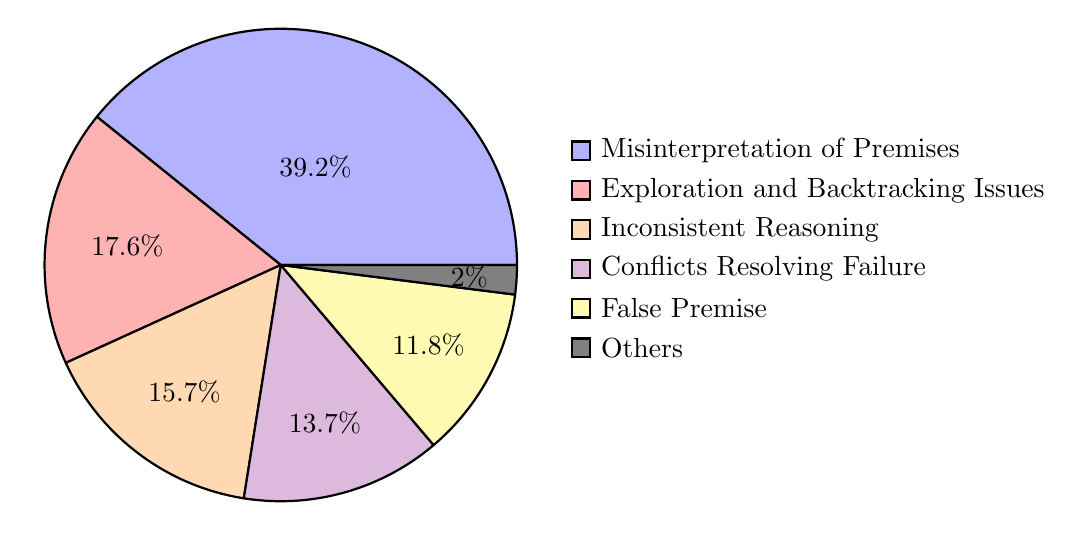
\begin{tikzpicture}
\pie[rotate=0, text = legend, color={blue!30, red!30, orange!30, violet!27, yellow!30, gray}]
 {39.2/Misinterpretation of Premises, 
 17.6/Exploration and Backtracking Issues, 
 15.7/Inconsistent Reasoning,
 13.7/Conflicts Resolving Failure,
 11.8/False Premise,
 2/Others
}  

% Exploration and Backtracking Issues                    17.647059
% Failure to Recognize, Resolve, or Explain Conflicts    13.725490
% False Premise                                          11.764706
% Inconsistent Reasoning                                 15.686275
% Misinterpretation of Premises                          39.215686
% Others (instruction following)                          1.960784
   
    \end{tikzpicture}
    }
\caption{Human analysis of error types.}
\label{fig:error_types}
\end{figure}

\pgfplotstableread{
Label Parent Sibling Multiple Invalid Child
o1 86	59	1	1	0
Gemini-FT 109 65 1 20 0
GPT-4o 157	7 7	107	1
GPT-3.5 146	63		76	50	97
Gemini-F 139	37		1	124	4
Qwen 215	21		0	121	1
    }\testdata
\begin{figure*}[t!]
    \centering
    \begin{subfigure}[b]{0.5\textwidth}
        \centering
        % \text{Performance Breakdown by Class} % Add the title here
        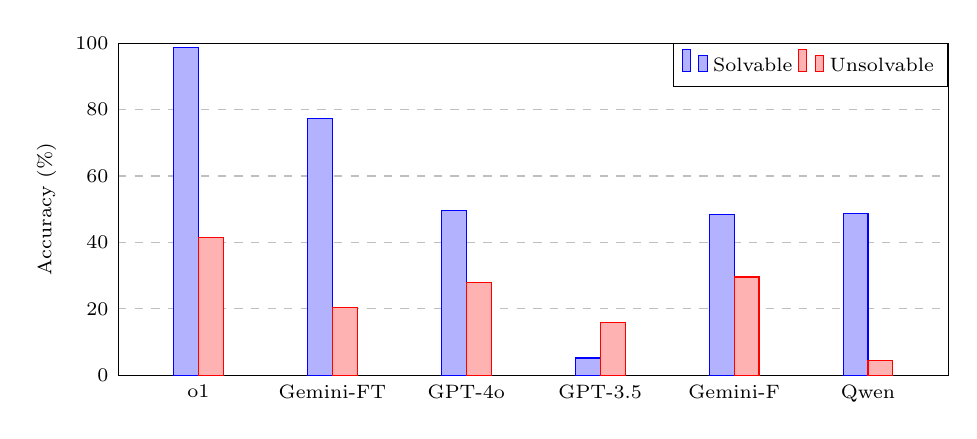
\begin{tikzpicture}
        \begin{axis}[
            width=\textwidth,
            height=5.8cm,
            ybar=0cm,
            bar width=9pt,
            ymax=100,
            ymin=0,
            xtick = {1,2,3,4,5,6},
            xticklabels = {o1, Gemini-FT, GPT-4o, GPT-3.5,  Gemini-F, Qwen},
            ylabel = {Accuracy (\%)},
            xtick pos = left,
            ytick pos = left,
            tickwidth=0mm,
            ymajorgrids = true,
            ytick={0,20,40,60,80,100},
            enlarge x limits=0.12,
            grid style=dashed, 
            legend style={at={(1,1)}, anchor=north east, legend columns=-1, font=\scriptsize},  
            xticklabel style={font=\scriptsize},
            yticklabel style={font=\scriptsize},
            ylabel style={font=\scriptsize}
        ]
        \addplot coordinates {(1,98.8) (2,77.2) (3,49.6) (4,5.2)  (5,48.4) (6,48.8)};    
        \addlegendentry{Solvable};
        \addplot coordinates {(1,41.6) (2,20.4) (3,28) (4,16) (5,29.6) (6,4.4)};    
        \addlegendentry{Unsolvable};

        % % Add annotations for improvement
        % \node at (axis cs:1,64.2) [anchor=south, xshift=17pt, yshift=2pt] {\scriptsize +2.5\%};
        % \node at (axis cs:2,79.5) [anchor=south, xshift=17pt, yshift=2pt] {\scriptsize +2.1\%};
    \legend{Solvable, Unsolvable}
    \end{axis}
    \end{tikzpicture}
    \vspace{-2mm}
    \caption{State-transition performance breakdown by class}
    \label{fig:ST-breakdown-by-class}
    \end{subfigure}%
    \hfill
    \begin{subfigure}[b]{0.5\textwidth}
        \centering
        % \text{MATH} % Add the title here
        \begin{tikzpicture}

    \begin{axis}[
        ybar stacked,
        width=\textwidth,
        height=5.8cm,
        ymin=0,
        ymax=600,
        bar width=12pt,
        xtick=data,
        ytick={0,250,500},
        ylabel = {Count},
        ylabel style={font=\scriptsize},
        legend style={at={(1,1)}, anchor=north east, legend columns=3, font=\scriptsize}, 
        reverse legend=true, 
        xticklabels from table={\testdata}{Label},
        xticklabel style={font=\scriptsize},
        yticklabel style={font=\scriptsize}]
    \addplot  table [y=Sibling, meta=Label, x expr=\coordindex] {\testdata};
    \addlegendentry{Sibling}
    \addplot  table [y=Parent, meta=Label, x expr=\coordindex] {\testdata};
    \addlegendentry{Backtracking failure}
    
    \addplot  table [y=Child, meta=Label, x expr=\coordindex] {\testdata};
    \addlegendentry{Unsolvable child}
    \addplot  table [y=Invalid, meta=Label, x expr=\coordindex] {\testdata};
    \addlegendentry{Invalid move}

    \addplot  table [y=Multiple, meta=Label, x expr=\coordindex] {\testdata};
    \addlegendentry{Multiple moves}
    % \addplot [
    %     ybar, % this makes it show the total for some reason
    %     nodes near coords,
    %     nodes near coords style={%
    %         anchor=south,%
    %     },
    % ] table [ y expr=0.00001, x expr=\coordindex] {\testdata};

    \end{axis}
    \end{tikzpicture}
    \vspace{-2mm}
    \caption{State-transition error type breakdown}
    \label{fig:ST-error}
    \end{subfigure}
    
    \caption{Performance breakdown and error analysis of state-transition in Sudoku.
    }
    \label{fig:ST-breakdown}
\end{figure*}


\subsection{State-Transition Performance Breakdown}

To understand models' behaviors during state transition, we breakdown the performance by class and count the common mistakes made by models.

The left chart of Figure~\ref{fig:ST-breakdown} shows the Sudoku state-transition performance breakdown for each class (solvable vs. unsolvable).
We observe that most models transit much better on solvable states than on unsolvable ones. The large gap indicates that models are better at proceeding forward from a valid state than backtracking. This might be attributed to a forward‐generation reasoning style of LLMs. This trend, however, does not apply to GPT-3.5, which shows significantly weak performance and tends to rely primarily on random guessing.

The right chart of Figure~\ref{fig:ST-breakdown} shows the errors typically made by models during state transition.
At solvable states, common errors include making multiple moves (Multiple Moves), violating Sudoku rules (Invalid Move), and transitioning to an unsolvable child state (Unsolvable Child).
At unsolvable states, two primary errors are: failing to return to the parent state (Backtracking Failure) and making an additional move to a sibling state after backtracking (Sibling). 
Among these errors, Backtracking Failure is the most frequent across all models. Models sometimes jump back more than one level (\eg to a grandparent state) or to a wrong state, indicating that LLMs struggle with step-by-step backtracking.
For reasoning models (o1 and Gemini-FT), transitioning to siblings is the second most frequent error. This error is due to violating the minimal move principle (Table~\ref{tab:node-edge-meaning}), highlighting weaknesses in their instruction-following capability.
For general models, they frequently commit an invalid move. This shows that general models often fail to adequately check Sudoku rules.


\subsection{Performance by Difficulty Level}

To understand the state-checking performance across difficulty levels, we plot the density diagrams of correct vs. incorrect predictions by the number of unfilled cells in the current Sudoku state. We observe that Sudoku states with fewer empty cells are more likely to be predicted correctly. As the number of unfilled cells increases, the problem becomes more complex and requires more exploration, and the proportion of incorrect predictions increases.

\begin{figure}[t!]
 \centering
    \includegraphics[width=0.95\linewidth]{assets/density-plot.pdf}
    \vspace{-2mm}
    \caption{Density plot of number of empty cells for correct vs. incorrect predictions.
    }
    \label{fig:difficulty}
\end{figure}



\section{Training Results}
As highlighted in \S\ref{sec:eval-results}, most models still lack state-checking and state-transition abilities, which are essential for reasoning. We hypothesize that training on these tasks can enhance performance on other reasoning-intensive tasks like math. To validate our hypothesis, we construct a training set consisting of state-checking and state-transition data from Sudoku, Graph Coloring, and Game of 24. We then train models on a mixture of this puzzle data and standard math data to test whether reasoning skills transfer beyond the puzzles themselves, ultimately improving overall mathematical reasoning.

\paragraph{Experimental setup.}
The puzzle states are easily verified, making it suitable for Reinforcement Learning. Specifically, we perform GRPO~\citep{shao2024deepseekmathpushinglimitsmathematical} on DeepSeek-R1-Distill-Qwen-1.5B and DeepSeek-R1-Distill-Qwen-7B~\citep{deepseekai2025deepseekr1incentivizingreasoningcapability}. We prepare $10,000$ samples from our puzzle dataset, and another $15,000$ samples from MetaMathQA~\citep{yu2024metamath}, a popular training set for mathematical reasoning. Other training details are reported in Appendix~\ref{sec:training-details}. Note that due to limited resources, we restrict the maximum completion length to 1024 in both training and evaluation.

\paragraph{Improvements on math benchmarks.}
We start with $2,000$ training samples, with a $1:1$ distribution between math and puzzle data. We compare with two baselines: first is the base model, second is training with entirely math samples. The results in Table~\ref{tab:main-training} show that combining puzzle data with MetaMath yields the highest accuracy on both GSM8K and MATH for both models, outperforming training on MetaMath alone. This consistent performance improvement suggests that the state-checking and state-transition logic of puzzle-solving generalize to more general mathematical problems, aligning well with our initial hypothesis.

\begin{table}[!t]
\small
\centering
\resizebox{1.0\linewidth}{!}{
\begin{tabular}{llrr}
\toprule
\textbf{Model} & \textbf{Data} & \textbf{GSM8K} & \textbf{MATH} \\
\midrule
\multirow{3}{*}{DeepSeek-R1-Distill-Qwen-1.5B} & None & 65.5 & 45.6 \\
& Math-only & 73.6 & 51.1 \\
& Mixed & \textbf{76.1} & \textbf{53.1} \\

\midrule
\multirow{3}{*}{DeepSeek-R1-Distill-Qwen-7B} & None & 79.7 & 63.2 \\
& Math-only & 82.3 & 70.7 \\
& Mixed & \textbf{87.4} & \textbf{71.4} \\

\bottomrule
\end{tabular}
}
\caption{\label{tab:main-training} Training with our puzzle data improves math reasoning on GSM8K and MATH.}
\end{table}


\paragraph{Analysis on the optimal ratio.} To investigate the optimal ratio between puzzle-based and math-based data, we vary the proportion of math samples from $0.4$ to $1.0$ in a combined training set of 10k samples. In Figure~\ref{fig:ratio}, the performance on GSM8K steadily improves as the math ratio increases, peaking at a ratio of  $0.8$. Beyond this point, increasing the math ratio further results in lower accuracy. This suggests that neither pure math training nor pure puzzle training is optimal. Instead, a balanced combination of puzzle-based and traditional math data provides the best performance. This indicates that our puzzle-based data though simple can complement the reasoning in standard math problems.
% These findings emphasize the complementary nature of puzzle and math data and underscore the need to carefully tune the training mixture for maximum benefit.

\paragraph{Analysis on the scaling effect.}
We investigate the scaling effect of using math-only and mixed math-puzzle data. We keep the ratio of math to $0.8$ in the mixed data. The results in Figure \ref{fig:scaling} show that, as we increase the number of training samples, both approaches benefit from scaling up. Noticeably, the mixed approach consistently outperforms math-only training starting from $5k$ samples. While math-only training shows diminishing returns or even a slight decline beyond $7.5k$ samples, the mixed approach continues to improve,  reaching an accuracy peak of $81.3\%$ with around $12.5k$ samples. 
This scaling effect suggests the great potential of our simple puzzle data for enhancing the overall reasoning capability of LLMs.


\begin{figure}
\centering
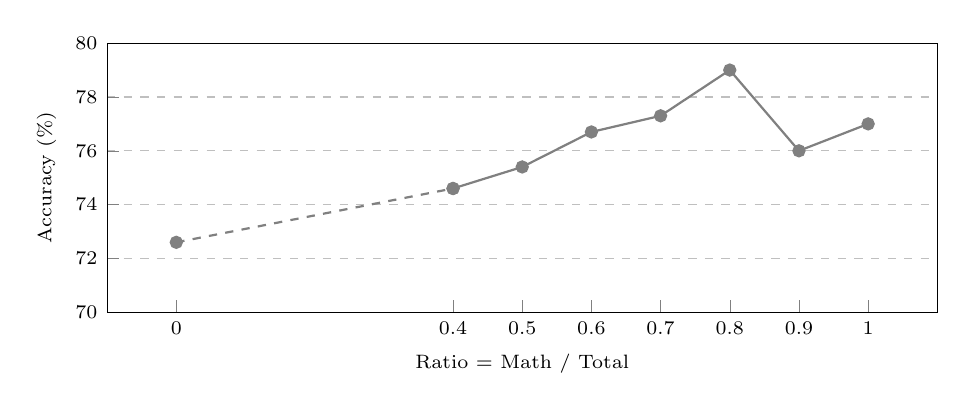
\begin{tikzpicture}
\pgfplotsset{width = \linewidth, height = 5cm}
    \begin{axis}[
        ymax=80,
        ymin=70,
        ylabel={Accuracy (\%)},
        xlabel={Ratio = Math / Total},
        xtick = {0,4,5,6,7,8,9,10},
        xticklabels = {0,0.4,0.5,0.6,0.7,0.8,0.9,1},
        xtick pos = left,
        ytick pos = left,
        ymajorgrids = true,
        grid style=dashed,
        xticklabel style={font=\scriptsize},
        xlabel style={font=\scriptsize},
        yticklabel style={font=\scriptsize},
        ylabel style={font=\scriptsize}
    ]
    \addplot [mark=*,mark options={solid}, dashed, color=gray, thick]
    plot coordinates {
    (0, 72.6) (4, 74.6) };
    \addplot [mark=*, color=gray, thick]
    plot coordinates {
    (4, 74.6) (5, 75.4) (6, 76.7) (7, 77.3) (8, 79) (9, 76) (10, 77) };
    \end{axis}
\end{tikzpicture}
\caption{The effect of training data mixing (Math v.s. Puzzle) on GSM8K using the 1.5B model.}
\label{fig:ratio}
\end{figure}

\begin{figure}
\centering
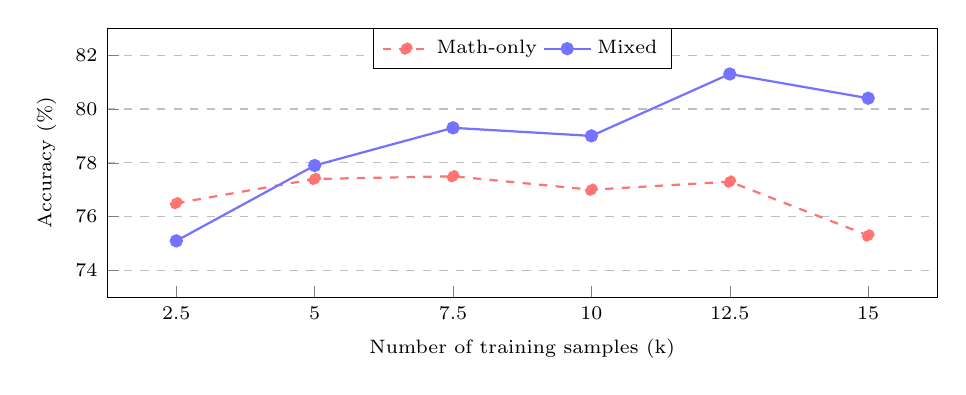
\begin{tikzpicture}
\pgfplotsset{width = \linewidth, height = 5cm}
    \begin{axis}[
        ymax=83,
        ymin=73,
        ylabel={Accuracy (\%)},
        xlabel={Number of training samples (k)},
        xtick = {1,2,3,4,5,6},
        xticklabels = {2.5,5,7.5,10,12.5,15},
        xtick pos = left,
        ytick pos = left,
        ymajorgrids = true,
        grid style=dashed,
        xticklabel style={font=\scriptsize},
        xlabel style={font=\scriptsize},
        yticklabel style={font=\scriptsize},
        ylabel style={font=\scriptsize},
        legend style={at={(0.5,1)}, anchor=north, legend columns=2, font=\scriptsize}, 
    ]
    % baseline
    \addplot [mark=*, dashed, color=red!55, thick]
    plot coordinates {
    (1, 76.5) (2, 77.4) (3, 77.5) (4, 77) (5, 77.3) (6, 75.3) };
    \addlegendentry{Math-only}
    \addplot [mark=*, color=blue!55, thick]
    plot coordinates {
    (1, 75.1) (2, 77.9) (3, 79.3) (4, 79) (5, 81.3) (6, 80.4)};
    \addlegendentry{Mixed}
    \end{axis}
\end{tikzpicture}
\caption{The scaling performance on GSM8K using the 1.5B model.}
\label{fig:scaling}
\end{figure}

\section{Related Work}
\paragraph{LLM Reasoning.}
Advancing the reasoning capabilities of large language models is a critical goal in natural language processing~\cite{wos1992automated,yang2018hotpotqa}. 
In recent years, LLMs, combined with prompting techniques such as Chain of Thought~\cite{wei2022chain}, Tree of Thought~\cite{yao2023tree}, and Self-Consistency~\cite{wang2023selfconsistency}, have shown remarkable performance in various reasoning tasks~\cite{cobbe2021training,srivastava2022beyond}.
Current evaluation methods focus mainly on the final accuracy in reasoning-intensive domains, including mathematics~\cite{cobbe2021training,math,chen-etal-2023-theoremqa,rein2023gpqa,VisAidMath}, coding~\cite{chen2021evaluating,austin2021program}, commonsense~\cite{mihaylov-etal-2018-suit,hendrycks2020measuring}, and logical reasoning~\cite{yao2023tree,long2023large}. However, as inference-time scaling gains importance~\cite{snell2024scaling,guo2025deepseek} and models are becoming more capable of reasoning, it is crucial to assess how effectively models perform reflection and correction during reasoning.
While \citet{tyagi-etal-2024-step} manually analyze the reasoning chains in logic puzzles, their approach lacks scalability.
Some studies~\cite{singh2024exposing,zeng2024mrben} evaluate how models handle reasoning mistakes, but these investigations often rely on rule-based mistakes that may be easily resolved by current LLMs. Moreover, these studies only assess reflection on past steps in a static manner.
In our work, we address these limitations by introducing two novel tasks designed to more accurately reflect models' capabilities in dynamic reasoning and error correction.


\paragraph{Puzzle Solving Tasks.}
Logic puzzles, which require deducing solutions from a set of rules~\cite{giadikiaroglou-etal-2024-puzzle}, are ideal for evaluating LLMs' reasoning capabilities as they rely minimally on prior knowledge~\cite{li-etal-2024-assessing-logical}.
Recent studies have explored LLMs on various puzzles with different emphases~\cite{mittal2024puzzlebench}, such as Sudoku~\cite{ishay2023leveraging,long2023large} for strategic thinking, Game of 24 ~\cite{ding2023everything,yao2023tree} for arithmetic calculations. Some investigate grid puzzles~\cite{dziri2024faith,tyagi-etal-2024-step}, crosswords~\cite{yao2023tree}, chess puzzles~\cite{feng2024chessgpt}, mazes~\cite{Noever2021PuzzleSW}, and Minesweeper~\cite{li-etal-2024-assessing-logical}.
However, evaluation remains primarily focused on final accuracy.




\section{Conclusion}
In this work, we introduced \framework, a novel logic-puzzle benchmark designed to comprehensively evaluate the reasoning capabilities of LLMs. Unlike existing benchmarks that focus mainly on final-answer accuracy, \framework delves into intermediate reasoning steps, specifically emphasizing state checking and transition actions. This fine-grained evaluation captures a model's ability to reflect, lookahead, and backtrack, which are vital aspects of human-like System 2 reasoning.
Our experiments reveal significant gaps between reasoning-oriented and general-purpose LLMs, emphasizing the need to consider reflection and correction for robust reasoning evaluation.
Furthermore, using puzzle-based data for training can enhance performance in broader mathematical tasks, highlighting the scalability of this approach and its potential to complement reasoning in standard math problems.


\section*{Limitations}
In our study, we use textual tables to represent puzzle states.
Our evaluation shows that models can reasonably understand this table format. However, there is potential to explore alternative representation formats, such as coordinates or images. The image format could be particularly valuable for facilitating the evaluation of multi-modal reasoning, offering a promising direction for future extensions of our work.

We adopt zero-shot CoT~\cite{kojima2022large} as the prompt format in all our evaluations. 
While advanced prompting techniques have the potential to enhance performance, their use might shift the focus away from evaluating the genuine reasoning capabilities of LLMs without excessive reliance on external assistance. By focusing on zero-shot CoT, we aim to provide a clearer evaluation of the models' inherent reasoning abilities. 


% Bibliography entries for the entire Anthology, followed by custom entries
\bibliography{custom}
% Custom bibliography entries only
% \bibliography{custom}
\clearpage
\appendix
% \onecolumn

\section{Appendix}

\subsection{Dataset Statistics}
\label{sec:dataset-statis}
Table~\ref{tab:dataset_statistics} presents the statistics for the four tasks, including the total number of questions, as well as the number of solvable and unsolvable states for each task. For grid puzzles, we can only sample 94 solvable states with unsolvable children, resulting in a somewhat imbalanced dataset. Nonetheless, we have maintained balance between solvable and unsolvable states for the remaining three puzzles.

% \begin{figure}[h!]
%  \centering
%     \includegraphics[width=\linewidth]{latex/assets/dataset_statistics.pdf}
%     % \vspace{-2mm}
%     \caption{Dataset statistics
%     }
%     \label{fig:dataset_stats}
%     % \vspace{-10pt}
% \end{figure}

\begin{table}[ht!]
\centering
 \resizebox{\linewidth}{!}{
\begin{tabular}{lccc}
\toprule
\textbf{Task} & \textbf{Questions} & \textbf{Solvable States} & \textbf{Unsolvable States} \\
\midrule
Sudoku & 51 & 250 & 250 \\
Graph Coloring & 51 & 250 & 250 \\
Game 24 & 98 & 250 & 250 \\
Grid Puzzles & 50 & 94 & 406 \\
\bottomrule
\end{tabular}}
\caption{Dataset Statistics}
\label{tab:dataset_statistics}
\end{table}

\subsection{Prompt Templates}
\label{sec:prompts}

Table~\ref{tab:prompts} shows the state checking and state transition prompts for a Sudoku example.






\subsection{Training Details}
\label{sec:training-details}
We train our models using GRPO based on OpenR1\footnote{https://github.com/huggingface/open-r1}. We use one GPU to run vLLM for faster generation and the remaining GPUs for training. The hyperparameters and training details are reported in Table~\ref{tab:params}.


\begin{table}[h]
    \centering
    \small
    % \resizebox{\linewidth}{!}{
    \begin{tabular}{lccccccc}
    \toprule
    % \textbf{}
    % % &\textbf{Value} \\
    % \midrule
    Learning rate & 4e-5 \\
    Warm up ratio & 0.1 \\
    Batch size & 112 \\
    Max prompt length & 1024 \\
    Max completion length & 1024 \\
    Training epochs & 1 \\
    Hardware & 8 H20 (120 GB) \\
    \bottomrule
    \end{tabular}
    % }
    \caption{Hyperparameter and training details.}
    \label{tab:params}
\end{table}

\subsection{Additional Experimental Results}
\label{sec:f-scores-full}

Table~\ref{tab:f-scores-full} reports the state-checking precision, recall, and F1 scores of models across four tasks. It is observed that o1 consistently outperforms all other models in detecting unsolvable states, as evidenced by the high recall and precision acorss tasks. Models like GPT-4o, Qwen2.5-Inst and Gemini-F are generally more precise when they predict unsolvability, but are limited by low recall in tasks like Sudoku and Grid Puzzles. GPT-3.5 generally struggles with both recall and precision, especially in more complex tasks like Sudoku.

\begin{table}[ht!]
\centering
\small
\resizebox{\linewidth}{!}{
\begin{tabular}{llrrrr}
\toprule
\textbf{Puzzle} & \textbf{Model} & \textbf{Recall} & \textbf{Precision} & \textbf{F1} \\
\midrule
\multirow{6}{*}{Sudoku} &
o1 & 73.2 & 86.7 & 79.4 \\
& GPT-4o & 6.4 & 80.0   & 11.9 \\
& GPT-3.5 & 28.0  & 49.0   & 35.6 \\
& Gemini-FT & 87.2 & 64.3 & 74.0 \\
& Gemini-F & 3.2 & 57.1 & 6.06 \\
& Qwen2.5-Inst & 4.8 & 75.0   & 9.02 \\
\midrule
\multirow{6}{*}{Game of 24} &
o1 & 95.6 & 99.2 & 97.4 \\
& GPT-4o & 95.6 & 75.9 & 84.6 \\
& GPT-3.5 & 54.8	& 56.6 &	55.7 \\
& Gemini-FT & 94.8 & 97.5 & 96.1 \\
& Gemini-F & 98.8 &	89.2 &	93.7 \\
& Qwen2.5-Inst & 97.6 &	82.2 &	89.2 \\
\midrule 
\multirow{6}{*}{Graph Coloring} 
& o1 & 93.1 & 95.9 & 94.5 \\ 
& GPT-4o & 44.8 & 57.8 & 50.5 \\ 
& GPT-3.5 & 27.4 & 53.5 & 36.3 \\ 
& Gemini-FT & 96.8 & 89.2 & 92.8 \\
& Gemini-F & 29.0 & 64.3 & 40.0 \\
& Qwen2.5-Inst & 25.8 & 73.6 & 38.2 \\
\midrule 
\multirow{5}{*}{Grid Puzzles} & o1 & 93.8 & 92.5 & 93.2 \\
& GPT-4o & 47.8 & 88.2 & 62.0 \\
& GPT-3.5 & 39.4 & 79.6 & 52.7 \\
& Gemini-FT & 91.6 & 94.7 & 93.1 \\
& Gemini-F & 24.4 & 94.3 & 38.7 \\
\bottomrule
\end{tabular}
}
\caption{\label{tab:f-scores-full}Precision, Recall and F1 scores of state checking task for all puzzles.}
\end{table}




\begin{table*}[ht]
    \centering
    \resizebox{\linewidth}{!}{
	\setlength{\tabcolsep}{0mm}{
            \begin{tabular}{p{20cm}}
            \toprule
            \textbf{State Checking} \\
            \midrule
                You are given a partially filled 9x9 Sudoku grid represented as a list of lists, where empty cells are represented as 0. Your task is to determine if this current state can lead to a solvable solution. Specifically, use lookahead techniques to determine if it's possible to fill the remaining cells according to standard Sudoku rules, ensuring that each row, column, and 3x3 subgrid contains unique numbers from 1 to 9. \\
                Additionally, you are provided with a previously explored next state that has been proven to be unsolvable. Use this information to avoid revisiting this failed path and leverage it to make a more informed decision about the current state.\\\\
                
                Current state: \textcolor{blue}{[[4, 1, 6, 9, 7, 2, 8, 3, 5], [7, 2, 3, 1, 8, 5, 6, 9, 4], [5, 9, 8, 3, 4, 6, 2, 1, 7], [6, 3, 5, 4, 1, 9, 7, 2, 8], [1, 8, 9, 2, 6, 7, 4, 5, 3], [2, 4, 7, 5, 3, 8, 1, 6, 9], [8, 7, 2, 6, 9, 3, 5, 4, 1], [3, 6, 0, 0, 5, 0, 0, 7, 2], [0, 0, 0, 0, 0, 4, 3, 8, 0]]}\\
                Explored next state that leads to an unsolvable path: \textcolor{blue}{[[4, 1, 6, 9, 7, 2, 8, 3, 5], [7, 2, 3, 1, 8, 5, 6, 9, 4], [5, 9, 8, 3, 4, 6, 2, 1, 7], [6, 3, 5, 4, 1, 9, 7, 2, 8], [1, 8, 9, 2, 6, 7, 4, 5, 3], [2, 4, 7, 5, 3, 8, 1, 6, 9], [8, 7, 2, 6, 9, 3, 5, 4, 1], [3, 6, 1, 0, 5, 0, 0, 7, 2], [0, 0, 0, 0, 0, 4, 3, 8, 0]]}\\
                Let's think step by step, considering the failed state to avoid unnecessary exploration. Do not solve using programming.\\
                Choose from (A) Solvable (B) Unsolvable. End your answer with "Answer: (A)" or "Answer: (B)". \\
            \midrule
            \textbf{State Transition} \\
            \midrule
            You are given an initial Sudoku puzzle S(0), followed by a sequence of progressive states leading to the current state S(i). Alongside each state, its solvability status L(*) is given. Your task is to determine the next state by making exactly one move, ensuring progress toward a valid solution. A valid Sudoku solution requires that each row, column, and 3x3 subgrid contains the numbers 1 to 9 without repetition.\\
            
            Additionally, you are provided with a previously explored next state that has been proven to be unsolvable. Use this information to avoid revisiting this failed path.\\

            A move is defined as either:\\
1. Filling: Replacing a 0 in exactly one empty cell with a value from 1 to 9.\\
2. Removing: Replacing a value in exactly one filled cell with 0.\\\\
Initial puzzle: \\
S(0) = \textcolor{blue}{[[0, 1, 0, 0, 7, 0, 8, 3, 0], [0, 2, 0, 0, 0, 0, 6, 0, 4], [5, 9, 0, 0, 0, 0, 0, 1, 0], [0, 0, 5, 0, 1, 9, 0, 0, 0], [1, 0, 0, 2, 6, 0, 0, 5, 3], [2, 4, 7, 0, 0, 8, 0, 0, 9], [0, 7, 0, 6, 9, 0, 0, 0, 1], [3, 0, 0, 0, 5, 0, 0, 7, 2], [0, 0, 0, 0, 0, 4, 3, 8, 0]]}\\
L(0) = \textcolor{blue}{Solvable} \\
Two moves ago:\\
S(i-2) = \textcolor{blue}{[[4, 1, 6, 9, 7, 2, 8, 3, 5], [7, 2, 3, 1, 8, 5, 6, 9, 4], [5, 9, 8, 3, 4, 6, 2, 1, 7], [6, 3, 5, 4, 1, 9, 7, 2, 8], [1, 8, 9, 2, 6, 7, 4, 5, 3], [2, 4, 7, 5, 3, 8, 1, 6, 9], [8, 7, 2, 6, 9, 3, 5, 0, 1], [3, 0, 0, 0, 5, 0, 0, 7, 2], [0, 0, 0, 0, 0, 4, 3, 8, 0]]}\\
L(i-2) = \textcolor{blue}{Solvable} \\
One move ago:\\
S(i-1) = \textcolor{blue}{[[4, 1, 6, 9, 7, 2, 8, 3, 5], [7, 2, 3, 1, 8, 5, 6, 9, 4], [5, 9, 8, 3, 4, 6, 2, 1, 7], [6, 3, 5, 4, 1, 9, 7, 2, 8], [1, 8, 9, 2, 6, 7, 4, 5, 3], [2, 4, 7, 5, 3, 8, 1, 6, 9], [8, 7, 2, 6, 9, 3, 5, 4, 1], [3, 0, 0, 0, 5, 0, 0, 7, 2], [0, 0, 0, 0, 0, 4, 3, 8, 0]]}\\
L(i-1) = \textcolor{blue}{Solvable} \\
Current state:\\
S(i) = \textcolor{blue}{[[4, 1, 6, 9, 7, 2, 8, 3, 5], [7, 2, 3, 1, 8, 5, 6, 9, 4], [5, 9, 8, 3, 4, 6, 2, 1, 7], [6, 3, 5, 4, 1, 9, 7, 2, 8], [1, 8, 9, 2, 6, 7, 4, 5, 3], [2, 4, 7, 5, 3, 8, 1, 6, 9], [8, 7, 2, 6, 9, 3, 5, 4, 1], [3, 6, 0, 0, 5, 0, 0, 7, 2], [0, 0, 0, 0, 0, 4, 3, 8, 0]]}\\
L(i) = \textcolor{blue}{Solvable} \\
Explored next state:\\
S(i+1) = \textcolor{blue}{[[4, 1, 6, 9, 7, 2, 8, 3, 5], [7, 2, 3, 1, 8, 5, 6, 9, 4], [5, 9, 8, 3, 4, 6, 2, 1, 7], [6, 3, 5, 4, 1, 9, 7, 2, 8], [1, 8, 9, 2, 6, 7, 4, 5, 3], [2, 4, 7, 5, 3, 8, 1, 6, 9], [8, 7, 2, 6, 9, 3, 5, 4, 1], [3, 6, 1, 0, 5, 0, 0, 7, 2], [0, 0, 0, 0, 0, 4, 3, 8, 0]]}\\
L(i+1) = \textcolor{blue}{Unsolvable} \\
Let's think step by step. Analyze the progress made so far and determine the immediate next move. 
End your answer with "Next state: \{grid\}", where \{grid\} is in the same python list format as the previous states.\\

            \bottomrule
            \end{tabular}

        }
    }
    \caption{
        Prompt templates for state checking and state transition in Sudoku.
    }
    \label{tab:prompts}
\end{table*}


\end{document}

